\documentclass{article}
\usepackage{graphicx}
\usepackage[colorlinks=false]{hyperref}
\usepackage{capt-of}
\usepackage{listings}

\begin{document}

\title{Hacking 10Base--T Ethernet\\for Underwater Optical Communication}
\author{UC the Fish}

\maketitle

\section{Introduction}

One of the funtional requirements for UC the Fish was modular optic communication,
or the communication system should be easy to integrate with devices that need to
communicate; a plug--and--play solution.

Nearly every modern computer has at least \mbox{10Base--T Ethernet} and
\mbox{USB 2.0} connectivity, so any ``modular'' communication attachement
should use one of these protocols--at least at its endpoints.
We chose to \mbox{10Base--T ethernet}, not just at the interfaces but to
send the ethernet signal itself through water in the form of intensity
of blue light.
This allowed us to focus on building blue light transmit and receive
hardware instead of attempting to develop light transmit/receive hardware
\textit{and} a modulation protocol + logic giving it USB endpoints.

Ethernet allows multiple stations to share a single medium,
which is appropriate for water because light spreads in every direction
and data cannot be multiplexed over different wavelegth channels. 
It includes hardware support for cyclic redundancy bit checking,
up to 16 retransmission attempts in the case of bit errors or disruption
of the medium, and at \mbox{10 MHz}, ethernet is fast enough 
for live streaming video.

Unlike USB, a temporary dissruption in the data link does not require
renegotiation time and application level link management.
Software applications can use the operating system to handle TCP protocol
when data integrity and delivery aknowledgement are necessary, instead
of writing custom code to ensure control commands reach the sub intact.

\section{Getting the Standard}

IEEE Std 802.3 is the standard for Ethernet communication.
It is freely available online but is so large it is split into multiple
sections.
The first section (only 555 pages!) is available at
\url{https://standards.ieee.org/getieee802/download/802.3-2012\_section1.pdf}.

\section[title]{Ethernet 101 \footnote{Or in other words, an Ethernet Preamble. Hehe.}}

Ethernet is a time--domain communication protocol for connecting any number of
machines via a single, shared medium.
Each \textit{station} is given a unique address when it is manufactured and
data is sent serially--1 bit at a time--in \textit{packets} between
stations.

\begin{center}
	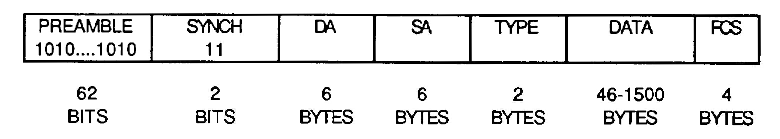
\includegraphics[width=0.75\textwidth]{ethernet-packet.pdf}
	\captionof{figure}{Format of an Ethernet Packet.}
\end{center}

Time sharing of the medium is done by all stations following
\textit{Carrier Sense Multiple Access with Collision Detection}
(CSMA/CD) protocol.
Only one station may transmit at a time and all stations must constantly
monitor the line, looking for packets addressed to them and seeing when
the line is open for transmission (CSMA).
After completion of a packet, all stations must wait an
\textit{interpacket gap} before transmitting a packet of their own.
If two stations transmit at the same time, both must detect a collision
and backoff for a period of time (/CD).
A pseudorandom exponential backoff algorithm is used to make repeat
collisions unlikely.
Retransmission is attempted up to 16 times when collisions occur.

\section{More Details from the Standard}



\section{Influence on Transmitter/Receiver Design}

\begin{enumerate}
\item The first component in the light transmitter input
and last component of the receiver output should be a 1:1, ethernet approved
transformer and standard RJ45 connector.
\item The input impedance of light transmitter must be $100\,\Omega$.
\item The bandwidth of both light transmitter and receiver must exceed $10\,MHz$
by several harmonics, and
\item their phase shift between $5\,MHz$ and $10\,MHz$ should be negligible.
\item The magnitude response of light transmitter + receiver in series,
to a $100\,ns$, $585\,mV$ step input, should be $\geq585\,mV$ when loaded by $100\,\Omega$.
\end{enumerate}

\section{Limitations for Underwater Communication}

There are two limitations associated with sending 10Base--T ethernet signals,
unmodified, through water by modulating light intensity.
Both limitations are related to the separation of transmit and receive signals
in 10Base--T networks how the stations detect collisions.

First, is the isolation of transmit and receive signals in twisted--pair media.

\begin{center}
	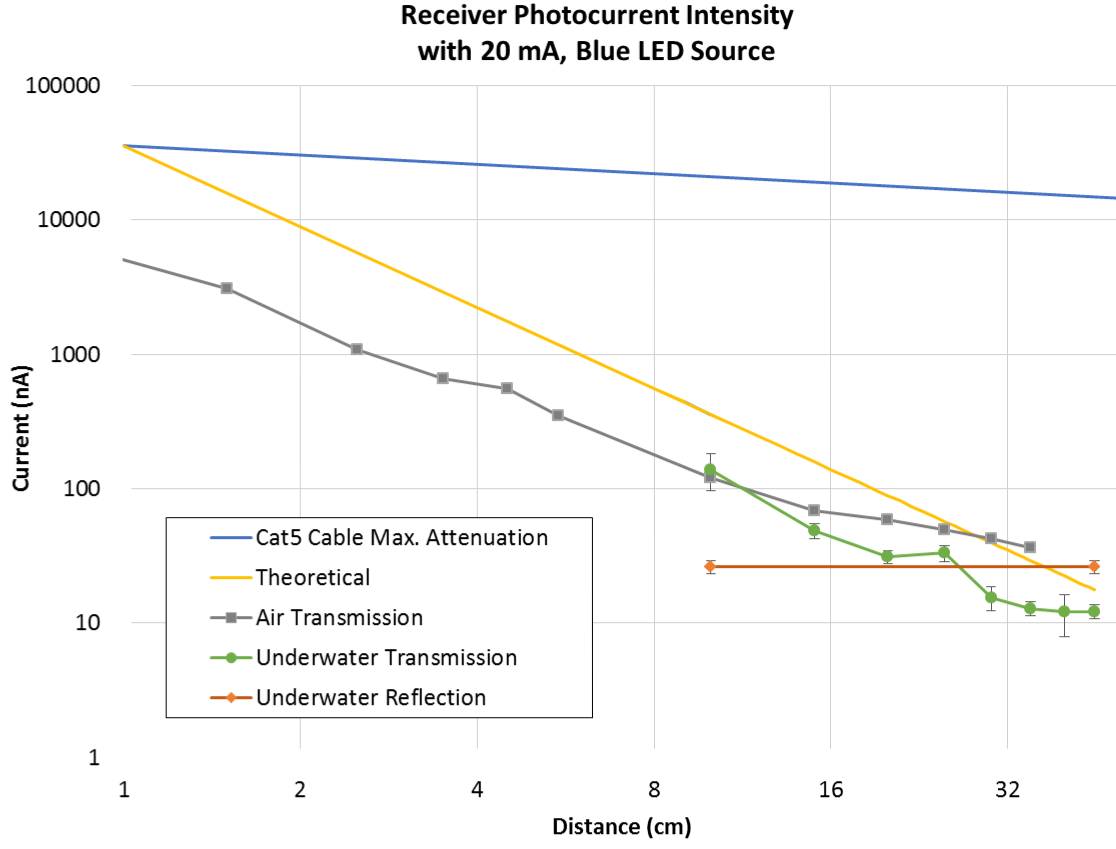
\includegraphics[width=0.8\textwidth]{crossover-point.pdf}
	\label{crossover-point}
	\captionof{figure}{The Crossover Point: distance at which reflected light from \mbox{station A's} own transmitter is more intense than
light arriving from far--away \mbox{station B's}.}
\end{center}

Second, the \textit{link integrity test} specified in the standard for twisted--pair media.

\appendix

\pagebreak
\section{Ethernet Test Scripts}

\lstinputlisting{Makefile}

\pagebreak
\lstinputlisting{broadcast_packet.c}

\pagebreak
\lstinputlisting{ethernet_listen.c}

\end{document}
